\begin{figure}[H]
\centering
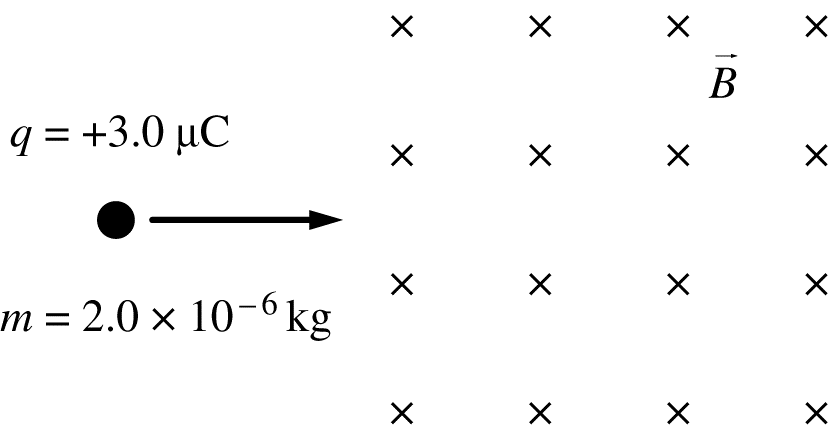
\includegraphics[scale=0.3]{images/img-012-028.png}
\end{figure}

% Multiple Choice Question 29
\begin{questions}\setcounter{question}{28}\question
A small object with a charge of $q=+3.0 \unit{\mu C}$ and a mass $m=2.0 \times 10^{-6} \unit{kg}$ enters a magnetic field of magnitude $B=0.20 \unit{T}$ directed into the page, as shown in the figure above. If the speed of the object is $1000 \unit{m/s}$, the object's acceleration at the moment it enters the field is most nearly

\begin{choices}
\choice zero because the velocity is perpendicular to the magnetic field
\choice $300 \unit{m/s^2}$ toward the bottom of the page
\choice $300 \unit{m/s^2}$ toward the top of the page
\choice $600 \unit{m/s^2}$ toward the bottom of the page
\choice $600 \unit{m/s^2}$ toward the top of the page
\end{choices}\end{questions}
